\teteSndMouv
\nomPrenomClasse
\titreActivite{Principe des actions réciproques}

%%%% evaluation
\pasCorrection{
\vspace*{-8pt}
\begin{tableauCompetences}
  ANA/RAI & Analyser les forces qui s'exercent sur un système. \\
  REA & Schématiser simplement une situation complexe. \\
  COM & Travailler en groupe en se répartissant des rôles. \\
\end{tableauCompetences}
}

%%%% objectifs
\begin{objectifs}
  \item Analyser et schématiser un système en mouvement
  \item Utiliser le principe d'inertie
  \item Comprendre le principe des actions réciproques
\end{objectifs}

%%%%
\begin{doc}{Forces qui se compensent}
  \begin{importants}
    On dit que les forces exercées sur un système \important{se compensent}, si leur somme vectorielle est nulle (égale à $\vv{0}$ le vecteur de norme nulle).
    
    \begin{wrapfigure}{r}{0.4\linewidth}
      \vspace*{-40pt}
      \begin{center}
        \begin{tikzpicture}
          % système
          \tikzSchemaPlanete [centre = $A$, rayon = 20pt, remplissage = couleurSec-200]
          % forces
          \tikzVecteur(0,0)(-1.7, -0.75) {$\vv{F}_1$} [left]
          \tikzVecteur(0,0)( 1.7,  0.75) {$\vv{F}_2$} [right]
        \end{tikzpicture}
      
        $\vv{F}_1 + \vv{F}_2 = \vv{0}$, les forces exercée sur le système $A$ se compensent.
      \end{center}
    \end{wrapfigure}
    
    La somme de deux vecteurs est nulle s'ils ont
    
    \begin{listePoints}
      \item \important{même point d'application,}
      \item \important{même direction,}
      \item \important{même norme ou valeur,}
      \item mais des \important{sens opposés.}
    \end{listePoints}
  \end{importants}
\end{doc}

\begin{doc}{Rappel de certaines forces}
  \begin{listePoints}
    \item Le poids $\vv{P}$, qui attire tous les objets vers le sol.
    \item La réaction du support $\vv{R}$, qui empêche les objets de traverser une surface.
    Elle est de même valeur que le poids, mais sa direction est perpendiculaire à la surface du support.
    \item Les frottements $\vv{f}$, qui s'opposent au mouvement d'un objet qui se déplace dans un fluide.
    Il \important{n'y a pas} de frottements sur un objet immobile.
  \end{listePoints}
\end{doc}


%%%%
\begin{doc}{Ballon lancé depuis un skateboard}
  \vspace*{-18pt}
  \begin{flushright}  
    \qrcode{https://edurl.fr/hYMcSxrq}
    % https://youtu.be/Kf0bBxmNeec?t=99}
  \end{flushright}
  
  \begin{multicols}{3}
    \centering
    \image{0.9}{images/mecanique/lancer_balle_reciproque_1.jpg}
    
    Avant le lancer
    
    \image{0.9}{images/mecanique/lancer_balle_reciproque_2.jpg}

    Pendant le lancer
    
    \image{0.9}{images/mecanique/lancer_balle_reciproque_3.jpg}

    Après le lancer
  \end{multicols}
\end{doc}


%%%
\problematique{Quelle est la force qui met en mouvement la personne sur le skateboard ?}

\question{
  Décrire le mouvement du système $A$ « personne sur le skateboard », avant, pendant et après le lancer du ballon. 
  Faire de même pour système $B$ « ballon » avant, pendant et après le lancer.
}{

}

\question{
  Lister toutes les forces qui s'exercent sur le système $A$ avant, pendant et après le lancer.
  Faire de même pour le système $B$.
}{

}

\schematisation Schématiser les forces qui s'exercent sur les systèmes A et B, avant, pendant et après le lancer du ballons. 